\documentclass[12pt,a4paper]{article}
\usepackage{fontspec}
\usepackage{amsmath, amssymb, amstext}
\usepackage{graphicx}
\usepackage{geometry}
\usepackage{xcolor}
\usepackage{fancyhdr}
\geometry{margin=1in}
\pagestyle{fancy}
\setlength{\headheight}{15pt} 
\lhead{کوییز درس فیزیک مدرن}
\chead{دانشکده فیزیک دانشگاه صنعتی خواجه نصیرالدین طوسی}
\rhead{۱۴۰۵/۰۳/22}
\usepackage{xepersian}
\settextfont{B Nazanin}

\begin{document}
	
	\begin{tabular}{|p{7cm}|p{7cm}|}
		\hline
		\textbf{نام و نام خانوادگی:} & \textbf{شماره دانشجویی:} \\
		\hline
	\end{tabular}
	
	
	\section*{سوالات:}
	\begin{enumerate}
		\item 
		
		جعبه‌ای به ابعاد \( a, b, c \) به حال سکون در نظر بگیرید. جرم سکون آن \( m_0 \) و چگالی سکون آن \( \rho_0 = \frac{m_0}{abc/25} \) است.
		
		\begin{enumerate}
			\item حجم جعبه را از نظر ناظری به دست آورید که نسبت به آن با سرعت \( u \) در امتداد محور \( x \) حرکت می‌کند.
			\item جرم آن از نظر ناظر چه قدر است؟
			\item چگالی جعبه بر حسب \( \rho_0 \) از نظر ناظر چه قدر است؟
		\end{enumerate}
		
		\begin{center}
			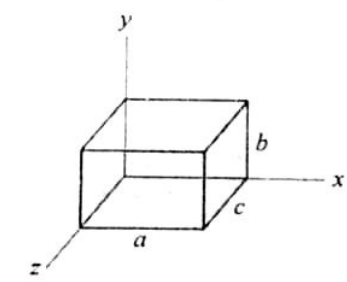
\includegraphics[width=0.5\textwidth]{../../images/image-E_3/image-3.png}
		\end{center}
		\item 
		الکترونی با انرژی جنبشی \lr{0.923} گیگا الکترون‌ولت در حال حرکت است. سرعت آن چقدر است؟
	\vspace{10pt}
	
	\textbf{موفق باشید.}
\end{enumerate}
\end{document}